\documentclass[10pt]{article}

\usepackage[a4paper, left=2cm, right=2cm]{geometry} % A4 paper size and thin margins

\usepackage{xcolor} % Required for specifying custom colours
\definecolor{grey}{rgb}{0.9,0.9,0.9} % Colour of the box surrounding the title

\usepackage{graphicx}
\usepackage[colorlinks=true, allcolors=black]{hyperref}
\usepackage{amsmath}
\usepackage{indentfirst}
\usepackage{blindtext}
\usepackage{multirow}
\setlength{\parindent}{2em}

\usepackage[utf8]{inputenc} % Required for inputting international characters
\usepackage[T1]{fontenc} % Output font encoding for international characters
\usepackage[sfdefault]{ClearSans} % Use the Clear Sans font (sans serif)
%\usepackage{XCharter} % Use the XCharter font (serif)
\usepackage{float}

\newcommand{\tabincell}[2]{\begin{tabular}{@{}#1@{}}#2\end{tabular}} 	

\begin{document}

%----------------------------------------------------------------------------------------
%	TITLE PAGE
%----------------------------------------------------------------------------------------

\begin{titlepage} % Suppresses displaying the page number on the title page and the subsequent page counts as page 1
	
	%------------------------------------------------
	%	Grey title box
	%------------------------------------------------
	
	\colorbox{grey}{
		\parbox[t]{1.1\textwidth}{ % Outer full width box
			\parbox[t]{1.02\textwidth}{ % Inner box for inner right text margin
				\raggedleft % Right align the text
				\fontsize{34pt}{40pt}\selectfont % Title font size, the first argument is the font size and the second is the line spacing, adjust depending on title length
				\vspace{0.7cm} % Space between the start of the title and the top of the grey box
				
				< Journey Assistant >\\
                Software Project Summary Report\\
                Version 1.0\\
				
				\vspace{0.7cm} % Space between the end of the title and the bottom of the grey box
			}
		}
	}
	
	\vfill % Space between the title box and author information
	
	%------------------------------------------------
	%	Author name and information
	%------------------------------------------------
	
	\parbox[t]{1\textwidth}{ % Box to inset this section slightly
		\raggedleft % Right align the text
		\large % Increase the font size
		{\Large Group Member}\\[4pt] % Extra space after name
        Yiwen Song\\
        Zhihui Xie\\
        Weizhe Wang\\
        Huangfei Jiang\\
        Haoping Chen\\
		% Institution Name\\[4pt] % Extra space before URL
		% \texttt{LaTeXTemplates.com}\\
		
		\hfill\rule{0.2\linewidth}{1pt}% Horizontal line, first argument width, second thickness
    }
    
	
\end{titlepage}

\newpage

\begin{center}
    {\LARGE Modification History}
    
    \begin{tabular}{|c|c|c|c|} 
        \hline 
        Date&Version&Description&Author\\
        \hline  
        2019-06-18&1.0&Finish the first version.&Haoping Chen\\
		\hline 
		& & & \\
		\hline
		& & & \\
		\hline
		& & & \\
		\hline
    \end{tabular}    
\end{center}

\newpage

\tableofcontents
\newpage

\section{Intruduction}
\subsection{Purpose}
This software orject summary report is aimed at summerizing the whole project of our ‘Journey Assistant’ App. The summery report will show the final result of our project, and summerize the experience and lessons we have learnt in this project. The document is used for summerize our project and gather experience for future work.

\subsection{Scope}
Software the document is applied on: Journey Assistant.

Characteristics, subsystems, models and codes related to the software all fit the contents of this the document.

\subsection{Definition}
The terms referred to in this document are defined in the project glossary document (Glossary.pdf).

\subsection{Bibliography}
\begin{itemize}
	\item[1.] <Object Oriented Software Engineering (Version 3)> (Tsinghua University Press)
	\item[2.] <Object Oriented Software Engineering Practice Guidelines> 
\end{itemize}

\subsection{Sketch}
This document icludes three parts: actual development results, evaluation of development work, experience and lessons. In actual develpment part, we summerize the product, cost, personnel, and etc of our project. In evaluation of development work, we look back on our development work in many aspects. Experience and lessons parts show the final reflection of our whole group. Different parts of this document complement and reference each other, and jointly shown the total outline of our ‘Journey Assistant’ App.

\section{Actual Development Result}
\subsection{Product}
\subsubsection{Android Client Program List}
Our Android client program list is shown in Table \ref{Android}.

\begin{table}[htb]
	\centering
	\begin{tabular}{|c|c|c|}
		\hline
		Package Name&Program Name &Size(KB)\\
		\hline
		\multirow{4}{*}{com.example.travelingagent.activity}
		&CheckItinerariesActivity.java &4 \\
		\cline{2-3}
		&CustomizationActivity.java &23 \\
		\cline{2-3}
		&FeedbackActivity.java &13 \\
		\cline{2-3}
		&Itinerary.java &2 \\
		\cline{2-3}
		&LoginActivity.java &8 \\
		\cline{2-3}
		&MainActivity.java &16 \\
		\cline{2-3}
		&RecommendationActivity.java &4 \\
		\cline{2-3}
		&RecommendationDisplayActivity.java &17 \\
		\cline{2-3}
		&RegisterActivity.java &6 \\
		\cline{2-3}
		&SavedItineraryDisplayActivity.java &15 \\
		\hline
		
		\multirow{4}{*}{com.example.travelingagent.entity}
		&Hotel.java &1 \\
		\cline{2-3}
		&Sight.java &1 \\
		\cline{2-3}
		&Spot.java &3 \\
		\cline{2-3}
		&User.java &2 \\
		\hline
		
		\multirow{4}{*}{com.example.travelingagent.protocol.api}
		&CustomizationClientApi.java &1 \\
		\cline{2-3}
		&ItineraryClientApi.java &1 \\
		\cline{2-3}
		&LoginClientApi.java &1 \\
		\cline{2-3}
		&RecommendationClientApi.java &1 \\
		\cline{2-3}
		&RegisterClientApi.java &1 \\
		\cline{2-3}
		&WeatherClientApi.java &1 \\
		\hline
		
		\multirow{4}{*}{com.example.travelingagent.protocol.entity}
		&ItemEntity.java &3 \\
		\cline{2-3}
		&LoginEntity.java &1 \\
		\cline{2-3}
		&ModeEntity.java &1 \\
		\cline{2-3}
		&RegisterEntity.java &1 \\
		\cline{2-3}
		&WeatherEntity.java &1 \\
		\hline
		
		\multirow{4}{*}{com.example.travelingagent.util.adapter}
		&FoldingCellListAdapter.java &6 \\
		\cline{2-3}
		&ItineraryRecyclerAdapter.java &6 \\
		\cline{2-3}
		&ModeAdapter.java &2 \\
		\cline{2-3}
		&RecyclerAdapter.java &6 \\
		\cline{2-3}
		&SpotAdapter.java &4 \\
		\hline
		
		com.example.travelingagent.util.easyFeedBack &EasyFeedback.java &2 \\
		\hline
		
		com.example.travelingagent.util.listener &ItemClickListener.java &1 \\
		\hline
		
		com.example.travelingagent.util.model &DataBean.java &3 \\
		\hline
		
		\multirow{4}{*}{com.example.travelingagent.util.viewHolder}
		&BaseViewHolder.java &1 \\
		\cline{2-3}
		&ChildViewHolder.java &2 \\
		\cline{2-3}
		&ItineraryParentViewHolder.java &4 \\
		\cline{2-3}
		&ParentViewHolder.java &4 \\
		\hline
		
		com.example.travelingagent.util &ReadFile.java &2 \\
		\hline
		\end{tabular}

		\caption{Android Client Program List}
		\label{Android}
\end{table}

\subsubsection{Server Program List}
Our server program list is shown in Table \ref{Server Program List}.

\begin{table}[htb]
	\centering

	\begin{tabular}{|c|c|c|}
		\hline
		Package Name&Program Name &Size(KB)\\
		\hline
		\multirow{4}{*}{com.test}
		&GetItinerary.java &4 \\
		\cline{2-3}
		&Gethotel.java &5 \\
		\cline{2-3}
		&Getsight.java &4 \\
		\cline{2-3}
		&Graph.java &4 \\
		\cline{2-3}
		&Hotel.java &2 \\
		\cline{2-3}
		&Itinerary.java &2 \\
		\cline{2-3}
		&Login.java &3 \\
		\cline{2-3}
		&Recommendation.java &5 \\
		\cline{2-3}
		&Register.java &3 \\
		\cline{2-3}
		&ReportMSG.java &3 \\
		\cline{2-3}
		&SaveItinerary.java &4 \\
		\cline{2-3}
		&SendItinerary.java &5 \\
		\cline{2-3}
		&Sight.java &1 \\
		\cline{2-3}
		&Simulation.java &4 \\
		\cline{2-3}
		&Spot.java &3 \\
		\cline{2-3}
		&Testjava.java &3 \\
		\cline{2-3}
		&Type.java &1 \\
		\cline{2-3}
		&User.java &1 \\
		\hline
		\end{tabular}
	\caption{Server Program List}
	\label{Server Program List}		
\end{table}

\subsubsection{Program System Version}
The system version of our program is shown in Table \ref{Program System Version}.

\begin{table}[htb]
	\centering

	\begin{tabular}{|c|c|c|c|}
		\hline
		Program System Name& Version &Description & Edit Time \\
		\hline
		\multirow{2}{*}{Journey Assistant}
		&v1.0 &Realize core use cases &5.17\\
		\cline{2-4}
		&v2.0 &Completely finished and pass the test & 6.17 \\
		\hline
		Journey Assistant Server& v1.0 & Completely finished and pass the test & 6.17\\
		\hline
		\end{tabular}
	\caption{Program System Version}
	\label{Program System Version}
\end{table}

\subsection{Main Functionality and Performance}
\subsubsection{Main Functionality List}
Our main functionality list is shown in Table \ref{Main Functionality List}.

\begin{table}[htb]
	\centering

	\begin{tabular}{c|c|c}
		\hline
		Main Functionality&Development Goal&Comment\\
		\hline
		Register&Realized&\\
		\hline
		Login&Realized&\\
		\hline
		Select Destination&Realized&\\
		\hline
		Set Preference&Realized&\\
		\hline
		View Map&Realized&\\
		\hline
		Recommendation&Realized&\\
		\hline
		Customiztion&Realized&\\
		\hline
		Check saved itineraries&Realized&\\
		\hline
		Feedback&Realized&\\
		\hline
   \end{tabular}
	\caption{Main Functionality List}
	\label{Main Functionality List}
\end{table}

\subsubsection{Main Performance List}
Our main performance list is shown in Table \ref{Main Performance List}.

\begin{table}[htb]
	\centering

	\begin{tabular}{c|c|c}
		\hline
		Main Performance&Development Goal&Comment\\
		\hline
		Response Time Requirement&Realized&The average response time is under 0.4s.\\
		\hline
		Throughput Requirement&Realized&Under 2500 requirements per second.\\
		\hline
		Capacity Requirement&Realized&\tabincell{c}{The maximum number of users \\and itineraries is around 140000.}\\
		\hline
		Resource Requirement&Realized&\tabincell{c}{The number of items in database is under 500000,\\
		the memory usage is no more than 300MB,\\
		and the bandwidth server needs is around 5Mbps}\\
		\hline
   \end{tabular}
	\caption{Main Performance List}
	\label{Main Performance List}
\end{table}

\subsection{Basic Procedure}
The core use cases are Recommedation Use Case and Customization Use Case. Sequence diagrams of them are shown below in Figure \ref{Recommendation Sequence Diagram} \& \ref{Customization Sequence Diagram}.

\begin{figure}[H]
	\centering
	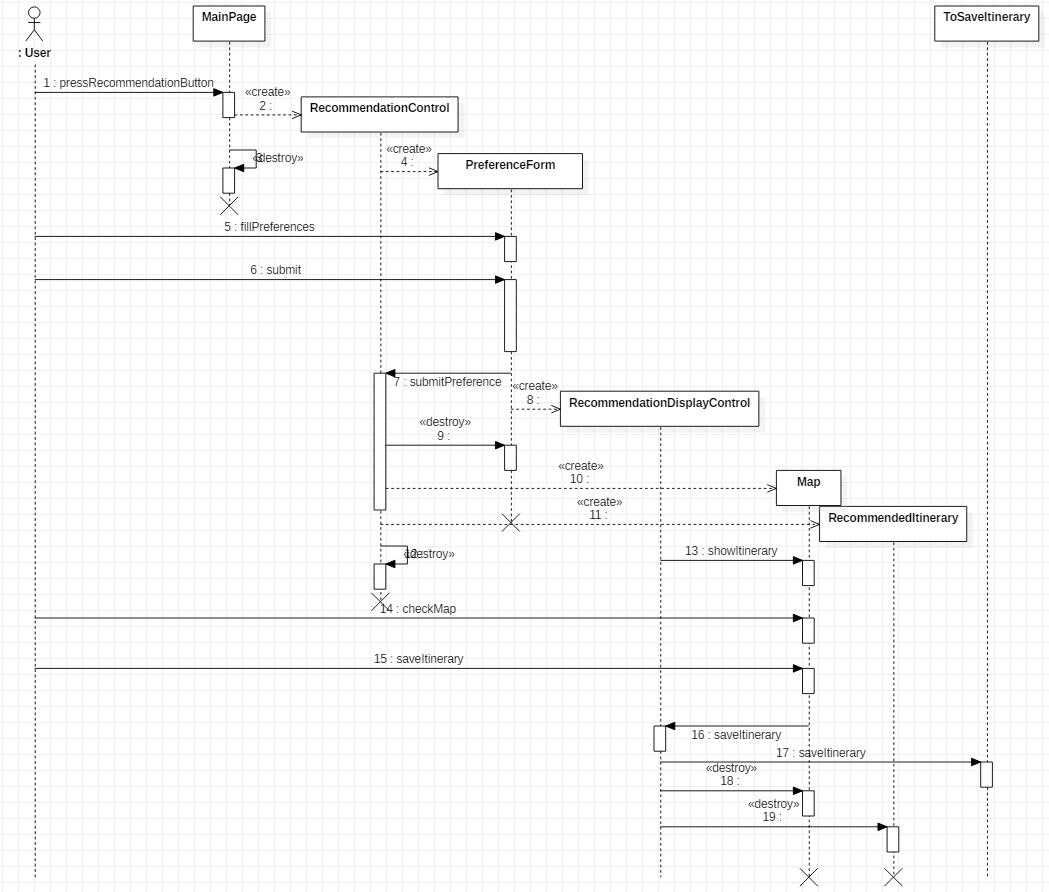
\includegraphics[width=14cm]{recommendation.png}
	\caption{Recommendation Sequence Diagram}
	\label{Recommendation Sequence Diagram}
\end{figure}
	
\begin{figure}[H]
	\centering
	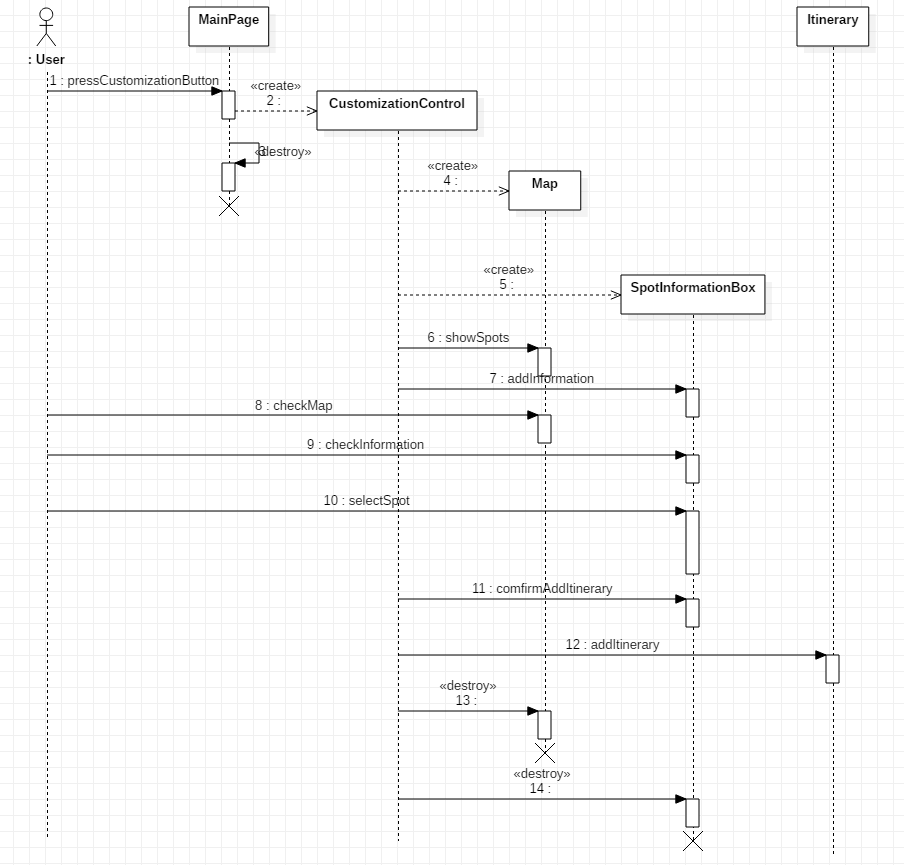
\includegraphics[width=14cm]{customization.png}
	\caption{Customization Sequence Diagram}
	\label{Customization Sequence Diagram}
\end{figure}

\subsection{Progress}
Our progress chart is shown in Table \ref{Progress Chart}:

\begin{table}[htb]
	\centering

	\begin{tabular}{|c|c|c|c|}
		\hline
		Milestone Events & Expected Deadline & Actual Finish Date & Schedule Variance\\
		\hline
		Software Requirement Specification Finished	& 4.20 & 4.15 & 5 days ahead \\
		\hline
		Software Architecture Document Finished	& 4.20 & 4.17 & 3 days ahead\\
		\hline
		Module Development Finished	&5.18	&5.16&	2 days ahead\\
		\hline
		System Integration Finished	&5.18	&5.18&	Exactly on time\\
		\hline
		System Test	&6.18	&6.17&	1 day ahead\\
		\hline
		Whole Project Finished	&6.18	&6.17&	1 day ahead \\
		\hline
		\end{tabular}

	\caption{Progress Chart}
	\label{Progress Chart}
\end{table}

Although it’s the first time for us to make the project, we keep pace with our schedule perfectly thanks to our careful plan and nice version control.

\subsection{Cost}
Since the whole project is carried out by team of students, there’s no actual cost.

\section{Development Work Evaluation}
\subsection{Evaluation of Production Efficiency}
In contrast to our origin plan, the actual production efficiency is even higher given such limited time.

\subsubsection{Actual Efficiency}
\begin{itemize}
	\item 3 months for system development
	\item Some repetitive operations
	\item 1200 lines of code in program per month per group member
	\item 4000 words in documentation per month per group member
	
\end{itemize}

\subsubsection{Origin Plan}
1000 lines of code and 3000 words per month per group member

\subsection{Evaluation of Production Quality}
BUG occur per 200 lines of code on average, the error rate is within estimate rate.

\subsection{Evaluation of Technique}
\paragraph{\underline{Github for Version Control}} It is helpful for cooperation of our group.

\paragraph{\underline{Client-Server Design Mode}} Front end is Android App, back end is Tomcat Server and SQLite3 database. This design mode accords with App development environment and is easy to manage.

\paragraph{\underline{MVC Design Mode}} Disassemble the system into Model, View and Controller. It is very common in Android development.

\paragraph{\underline{Three Layers of System Architecture}}
\subparagraph{User Interface Layer} UI of App

\subparagraph{Application Logic Layer} control the realization of functionalities

\subparagraph{Storage Layer} responsible for data storage, retrieval and searching


\paragraph{\underline{API Usage}}The usage of API enriches the content of our project.
\begin{itemize}
	\item Baidu Map API for displaying recommendation result and trip customization
	\item Meizu Weather API for getting weather information.
\end{itemize}

\paragraph{\underline{Markov Decision Making Process in Trip Recommendation}} It’s an effective way to recommend different trips based on user biases.

\subsection{Error Analysis}
\begin{itemize}
	\item When Android Studio can not compile the project, the error is that the gradle version is not the latest, and also dependencies are not added in the gradle.
	\item When crash happens on the App, the reason is that there’s something wrong with Intent communication
	
\end{itemize}

\section{Experience and Lessons}
\subsection{Experience}
\subsubsection{Schedule}
We should foresee the problems we may confront when making plans, and reserve time for each stage at the beginning.

\subsubsection{Requirement}
User requirements should be fullycollected so that we can make better analysis and development.

\subsubsection{Design}
Use UML in project design, which provide perfect guiding function.

\subsubsection{Technique} 
Use of different APIs enrich the content of our project.

\subsection{Lessons}
What we did not do very well is version control. Although we use Github to help control our version, we sometimes did not update our codes in github, which brings out the problem that one file may be modified by more than one group member, adding to integration workload of our project. So wo should commit our change in github once we have made some changes.

\end{document}
